\documentclass{beamer}
\usepackage{epstopdf}
\usepackage{amssymb,amsmath}
\usepackage{hyperref}
\definecolor{links}{HTML}{2A1B81} 
\hypersetup{colorlinks,linkcolor=,urlcolor=links}
%\usepackage{xcolor}
\usepackage{pgfplots}
%\usepackage[usenames,dvipsnames]{color}
\usetikzlibrary{arrows,shapes,positioning}
\definecolor{BrickRed}{RGB}{178,34,34}



\usepackage{graphicx}
\usepackage{multirow}
\usepackage[overlay]{textpos}
\usetheme{Copenhagen}
\usecolortheme{beaver}
\usecolortheme{orchid}
\setbeamertemplate{navigation symbols}{\insertframenumber} 
\colorlet{lightgray}{gray!40}
\setbeamercolor{postit}{fg=purple,bg=lightgray}
% \usepackage{beamerthemesplit} // Activate for custom appearance


\addtobeamertemplate{frametitle}{}{%
\begin{textblock*}{50mm}(.92\textwidth,-0.8cm)
\includegraphics[height=0.55cm,width=1.5cm]{/Users/caitlinmalone/Documents/ATLAS/slac_logo.pdf}
\end{textblock*}}

% \usepackage{beamerthemesplit} // Activate for custom appearance

\title{Higgs Bosons Decaying to Fermions in ATLAS and CMS}
%\subtitle{Higgs Couplings 2013, Frieburg}
\author{Caitlin Malone, SLAC}
\institute{on behalf of the ATLAS Collaboration\\Higgs Couplings 2013, Frieburg\\14 October 2013 }
\date{}

\begin{document}

\frame{\titlepage}


\begin{frame}{Introduction}
	\begin{itemize}
		\item Newly discovered Higgs boson must be studied
		\item Has a mass (approx. 126 GeV) that decays in many channels
		\item Discovered in the $\gamma \gamma$ and heavy vector boson channels
		\item Large BR to bb
		\item $\tau \tau$ also in the picture
		\item $\mu \mu$ rounds out the SM fermionic channels
	\end{itemize}
\end{frame}


\begin{frame}{Production Channels}
	\begin{columns}[c]
	\column{0.25\textwidth}
	\column{0.5\textwidth}
		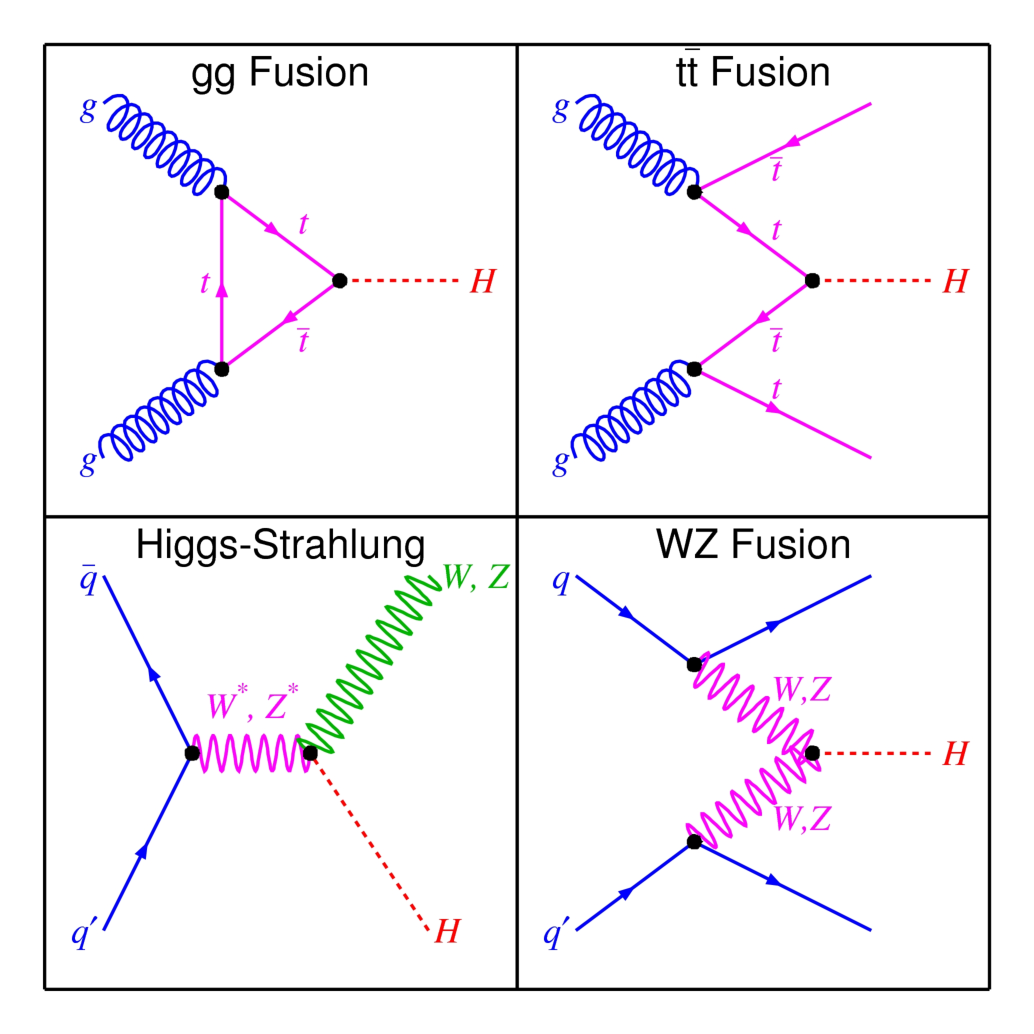
\includegraphics[width=\textwidth]{/Users/caitlinmalone/Documents/ATLAS/HiggsCouplings2013/figures/higgs_feyn_pp.pdf}
	\column{0.25\textwidth}
	\end{columns}
\end{frame}


\begin{frame}{Branching Fractions}
	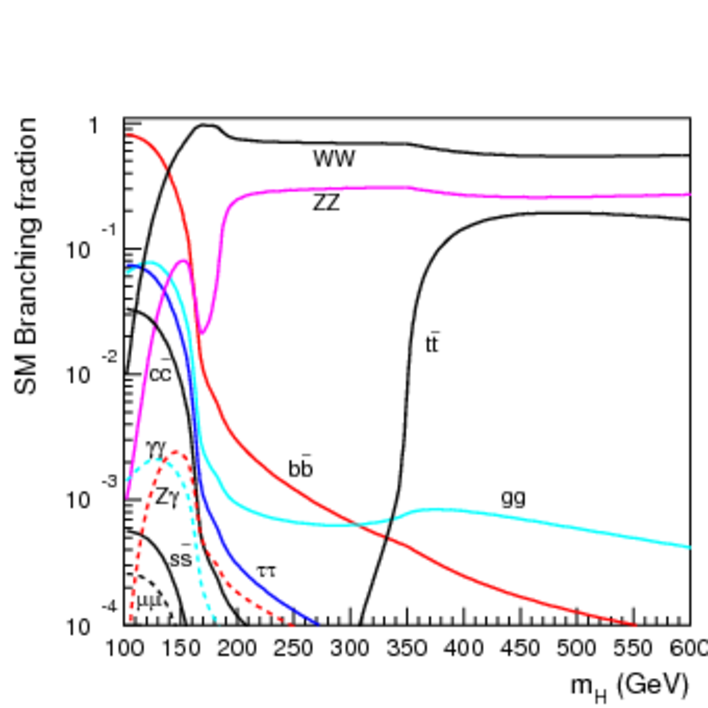
\includegraphics[width=0.7\textwidth]{/Users/caitlinmalone/Documents/ATLAS/HiggsCouplings2013/figures/h_br_sm.pdf}
\end{frame}





\begin{frame}{$H\rightarrow \tau \tau$ Motivation}
	\begin{itemize} \scriptsize
		\item Direct coupling to lepton sector
		\item 4th channel for observation, after vector bosons and $\gamma \gamma$
		\item 6.3\% branching ratio at $m_H$=125 GeV
%		\item Organized by $\tau$ decays: $\tau_{lep}\tau_{lep}$, $\tau_{lep}\tau_{had}$, $\tau_{had}\tau_{had}$ where $lep=\mu,e$
%		\item 0-jet, 1-jet, VBF in lep/had
	\end{itemize}
	\begin{columns}
		\column{0.33\textwidth}
		$\tau_{lep}\tau_{had}$
		\column{0.33\textwidth}
		$\tau_{lep}\tau_{lep}$
		\column{0.33\textwidth}
		$\tau_{had}\tau_{had}$
	\end{columns}
\end{frame}





\begin{frame}{$H \rightarrow \tau \tau$: Overview of Analyses}
	\begin{table}
%		\scriptsize
		\begin{tabular}{c | c | c | c | c | c | c}
		
		
		 & VBF & Boosted & VH & 1-jet & ttH & 0-jet$^*$\\ \hline \hline
		 
				
			$\mu \tau_{had}$ &
			
\includegraphics[width=0.05\textwidth]{figures/atlas_logo.pdf} 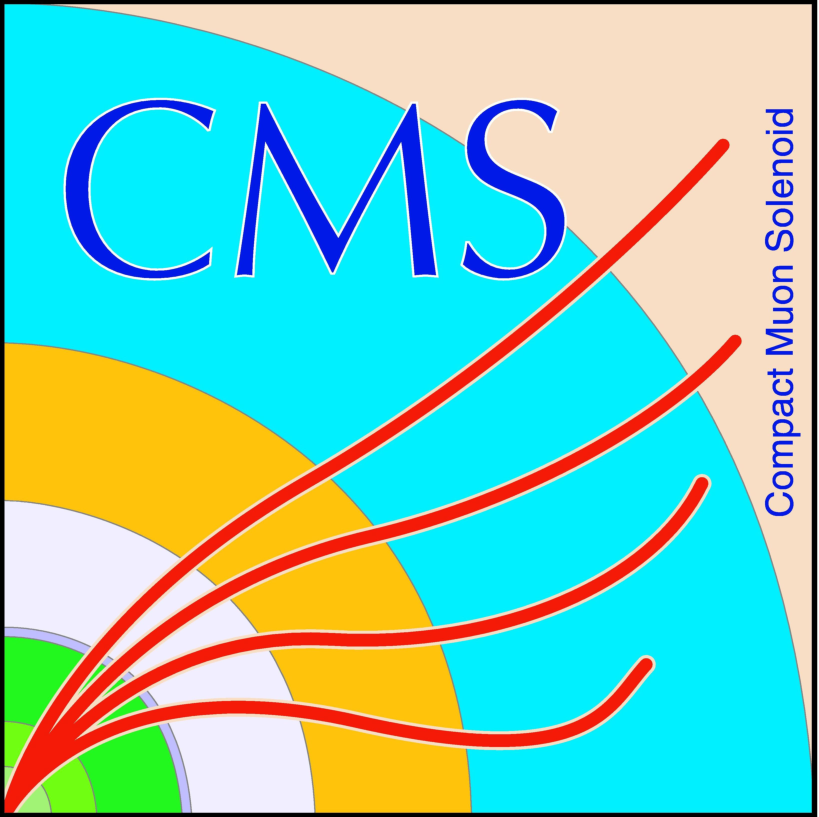
\includegraphics[width=0.05\textwidth]{figures/cms_logo.pdf} &
			
\includegraphics[width=0.05\textwidth]{figures/atlas_logo.pdf} &
			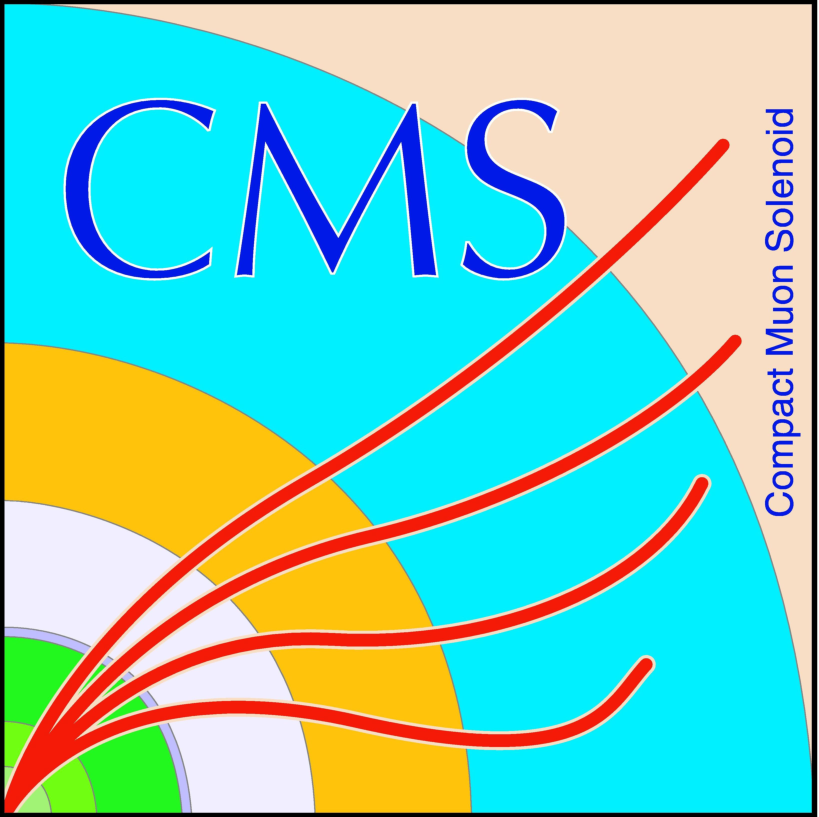
\includegraphics[width=0.05\textwidth]{figures/cms_logo.pdf}&

			
\includegraphics[width=0.05\textwidth]{figures/atlas_logo.pdf} 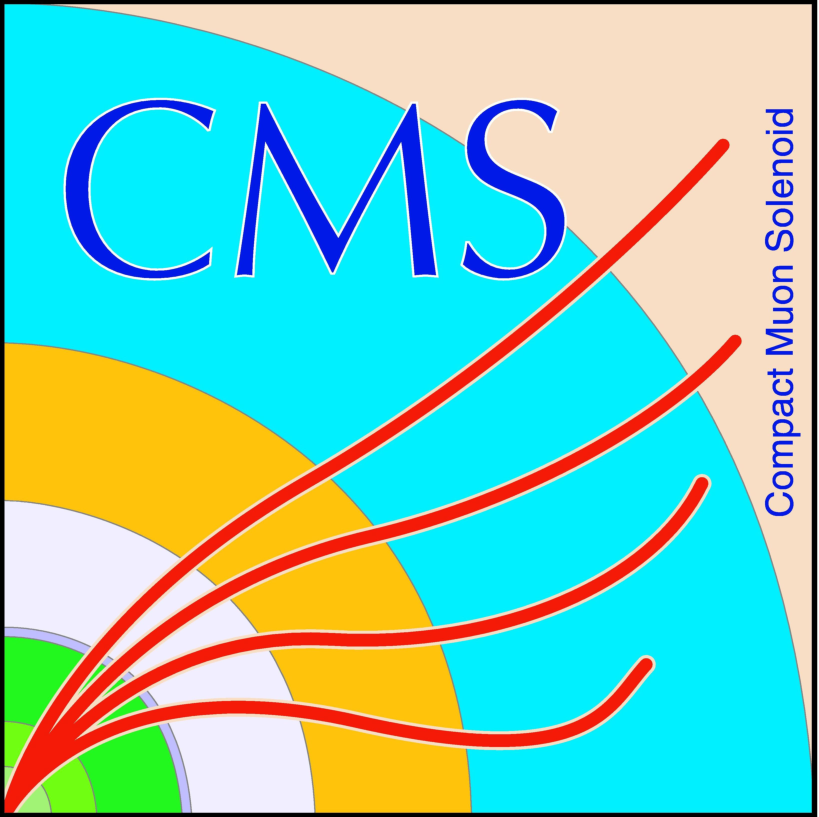
\includegraphics[width=0.05\textwidth]{figures/cms_logo.pdf} &
			&
			
\includegraphics[width=0.05\textwidth]{figures/atlas_logo.pdf} 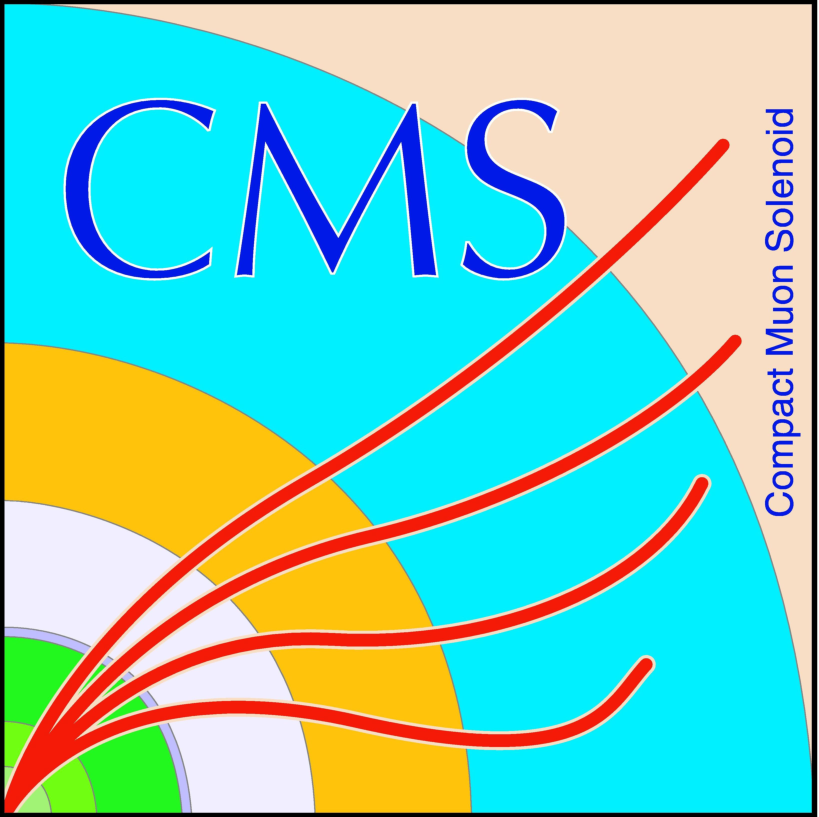
\includegraphics[width=0.05\textwidth]{figures/cms_logo.pdf} 	
			\\	
			$e \tau_{had}$ &
			
\includegraphics[width=0.05\textwidth]{figures/atlas_logo.pdf} 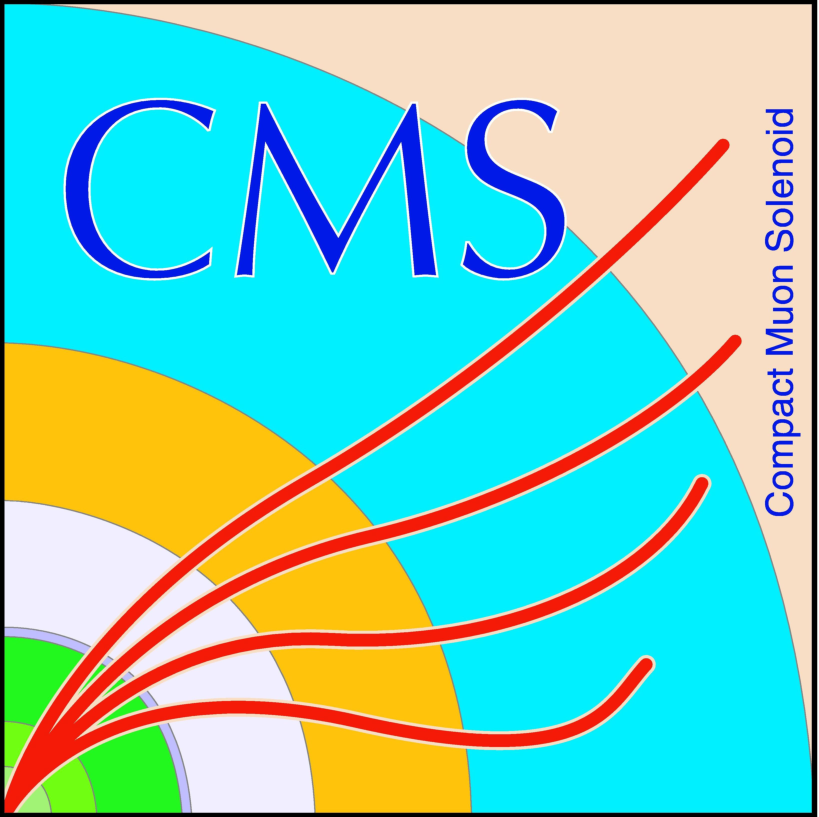
\includegraphics[width=0.05\textwidth]{figures/cms_logo.pdf} &
			
\includegraphics[width=0.05\textwidth]{figures/atlas_logo.pdf} &
			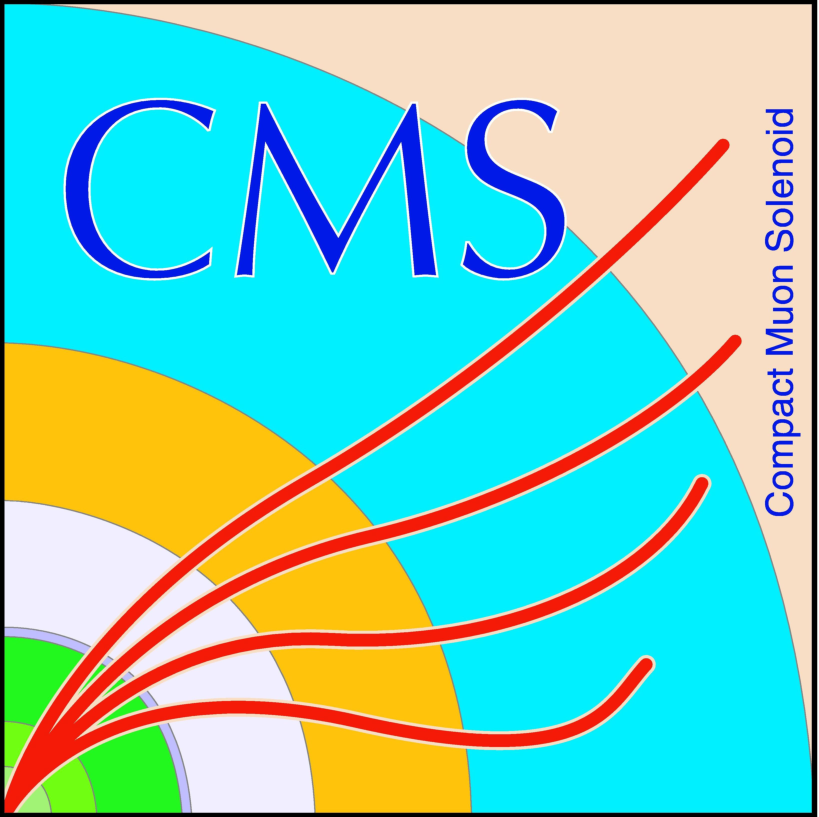
\includegraphics[width=0.05\textwidth]{figures/cms_logo.pdf} &
			
\includegraphics[width=0.05\textwidth]{figures/atlas_logo.pdf} 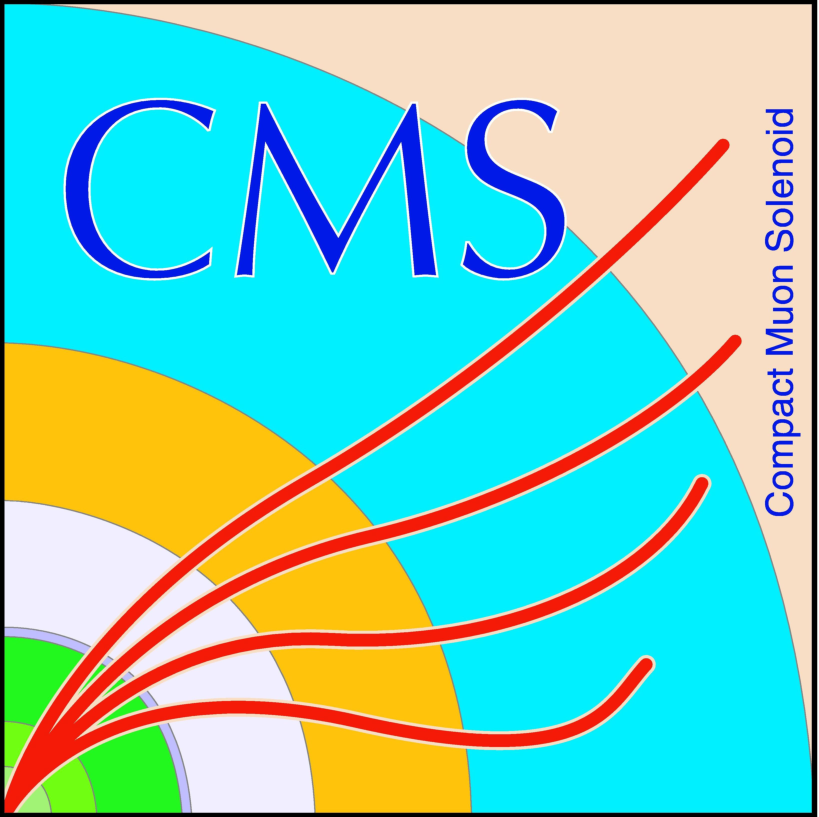
\includegraphics[width=0.05\textwidth]{figures/cms_logo.pdf} &
			&
			
\includegraphics[width=0.05\textwidth]{figures/atlas_logo.pdf} 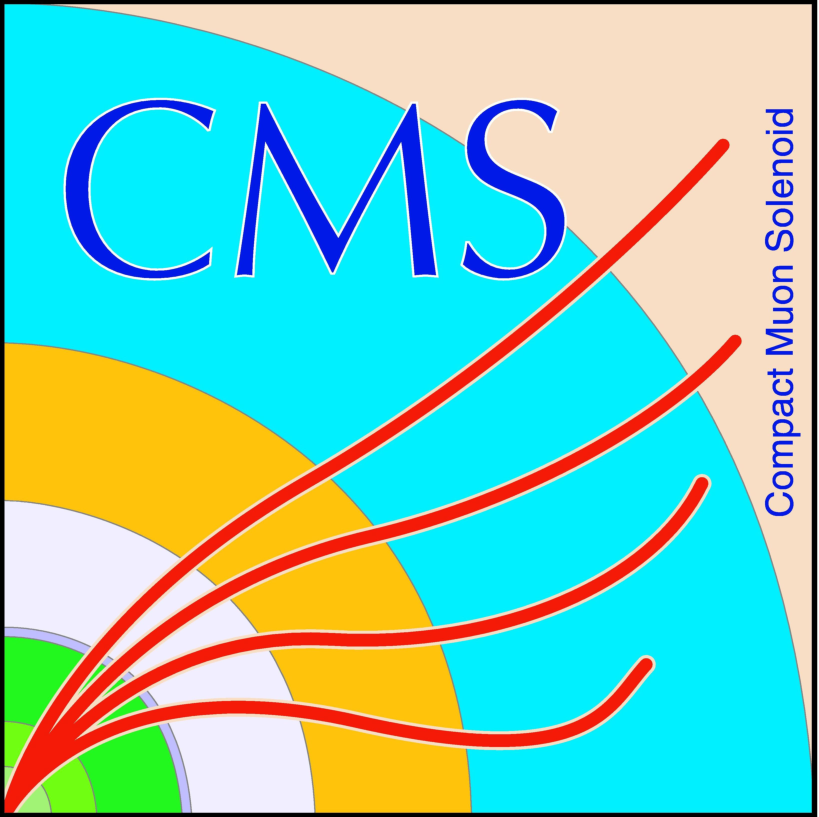
\includegraphics[width=0.05\textwidth]{figures/cms_logo.pdf} 	
			\\	
			
			 
			\hline		
			$\mu e$ &
			
\includegraphics[width=0.05\textwidth]{figures/atlas_logo.pdf} 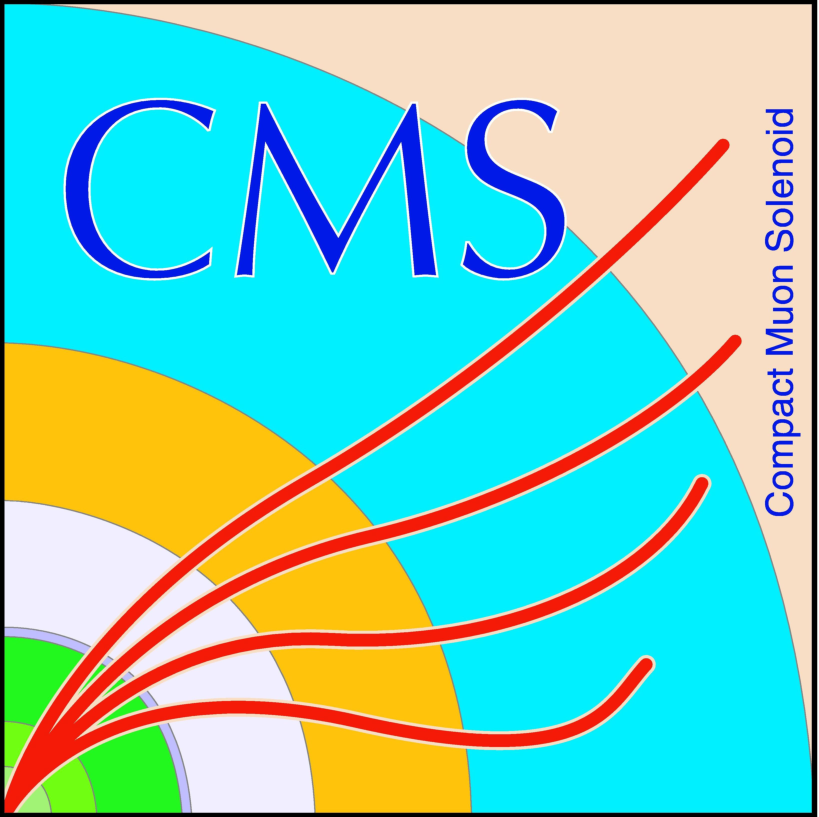
\includegraphics[width=0.05\textwidth]{figures/cms_logo.pdf} &
			
\includegraphics[width=0.05\textwidth]{figures/atlas_logo.pdf} &
			
\includegraphics[width=0.05\textwidth]{figures/atlas_logo.pdf} 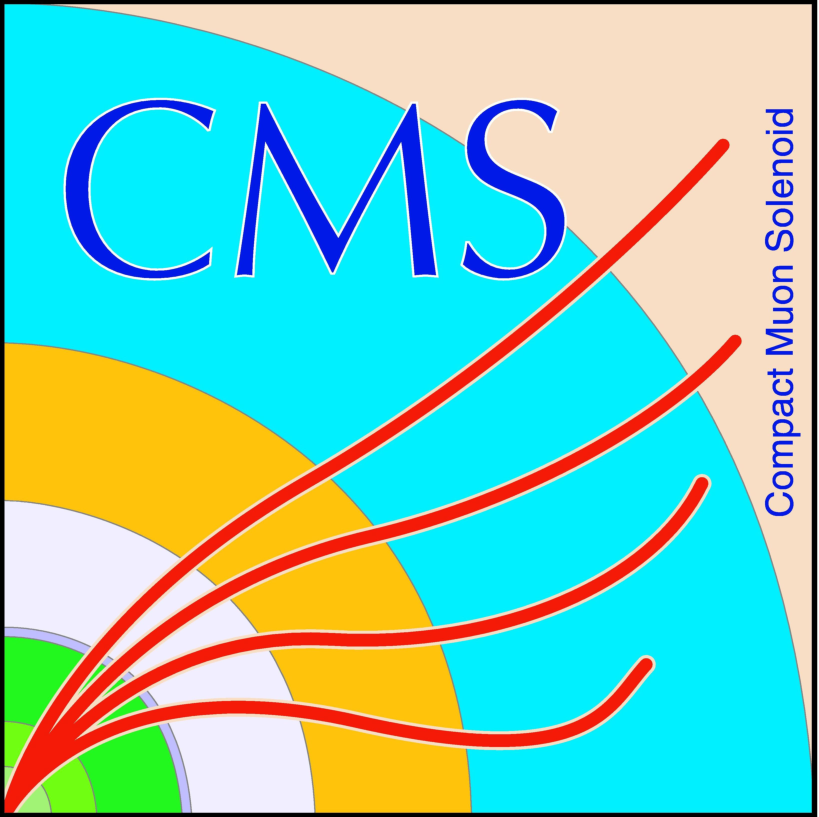
\includegraphics[width=0.05\textwidth]{figures/cms_logo.pdf}&
			
\includegraphics[width=0.05\textwidth]{figures/atlas_logo.pdf} 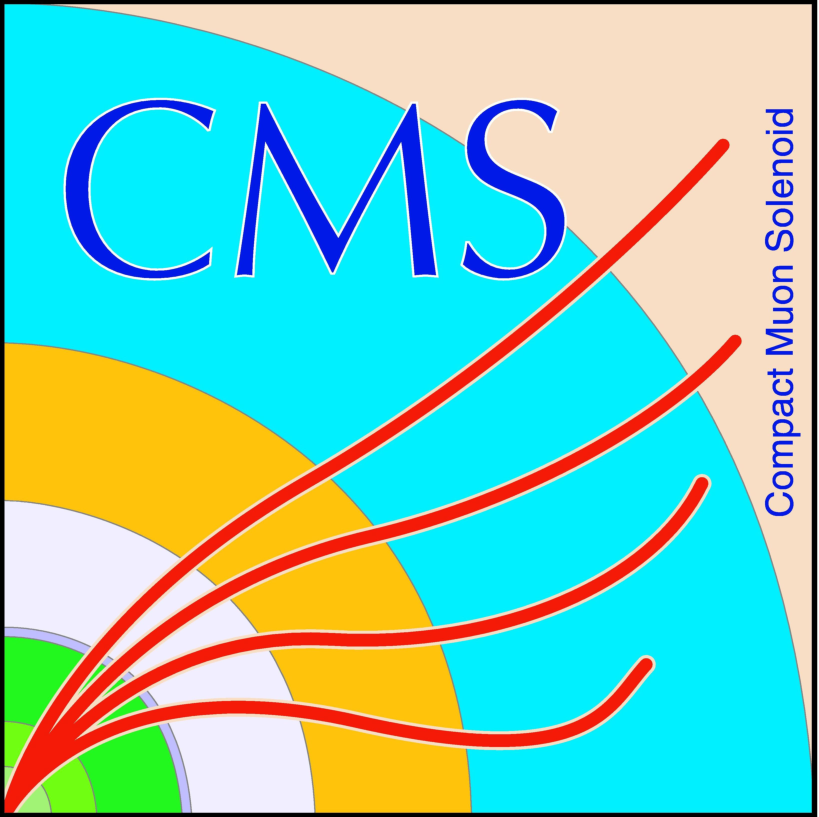
\includegraphics[width=0.05\textwidth]{figures/cms_logo.pdf} &
			&
			
\includegraphics[width=0.05\textwidth]{figures/atlas_logo.pdf} 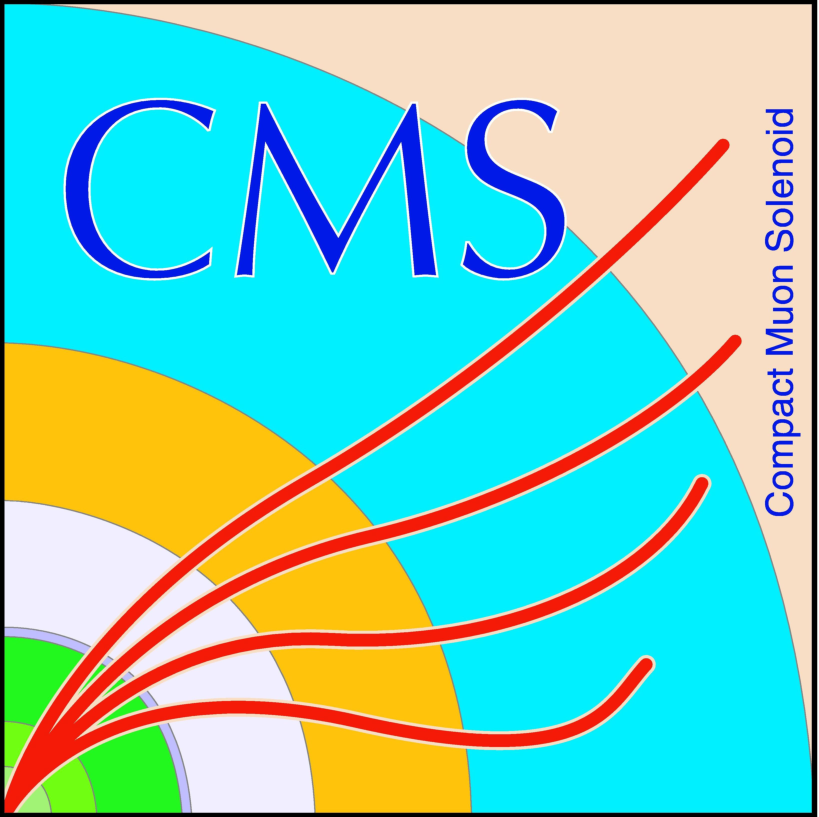
\includegraphics[width=0.05\textwidth]{figures/cms_logo.pdf} 	
			\\
			$\mu\mu$ &
			
\includegraphics[width=0.05\textwidth]{figures/atlas_logo.pdf} 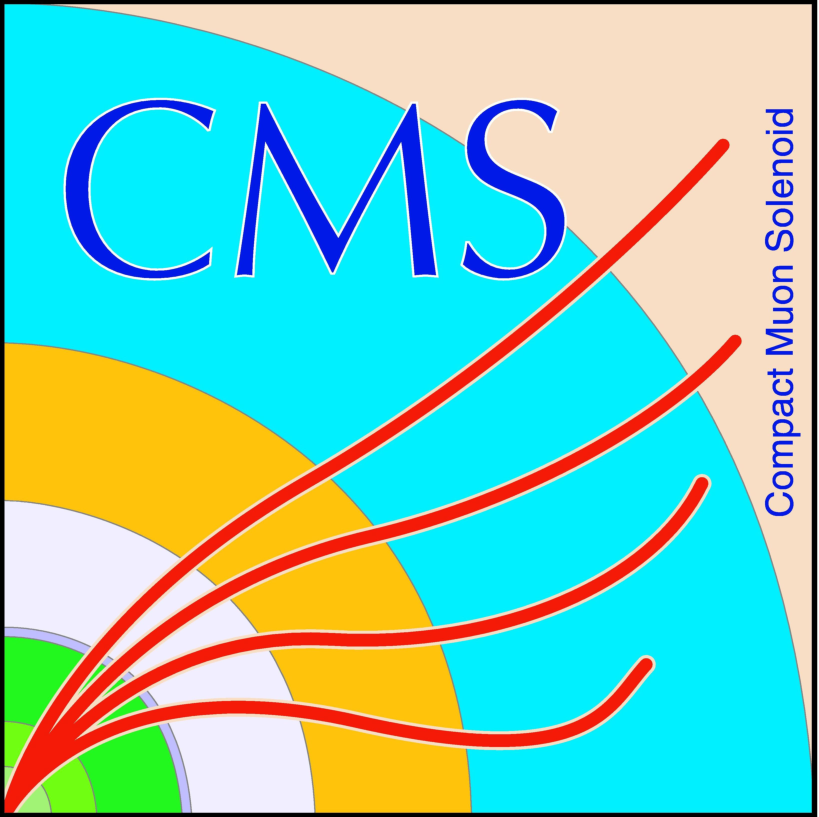
\includegraphics[width=0.05\textwidth]{figures/cms_logo.pdf} &
			
\includegraphics[width=0.05\textwidth]{figures/atlas_logo.pdf} &
			
\includegraphics[width=0.05\textwidth]{figures/atlas_logo.pdf} &
			
\includegraphics[width=0.05\textwidth]{figures/atlas_logo.pdf} 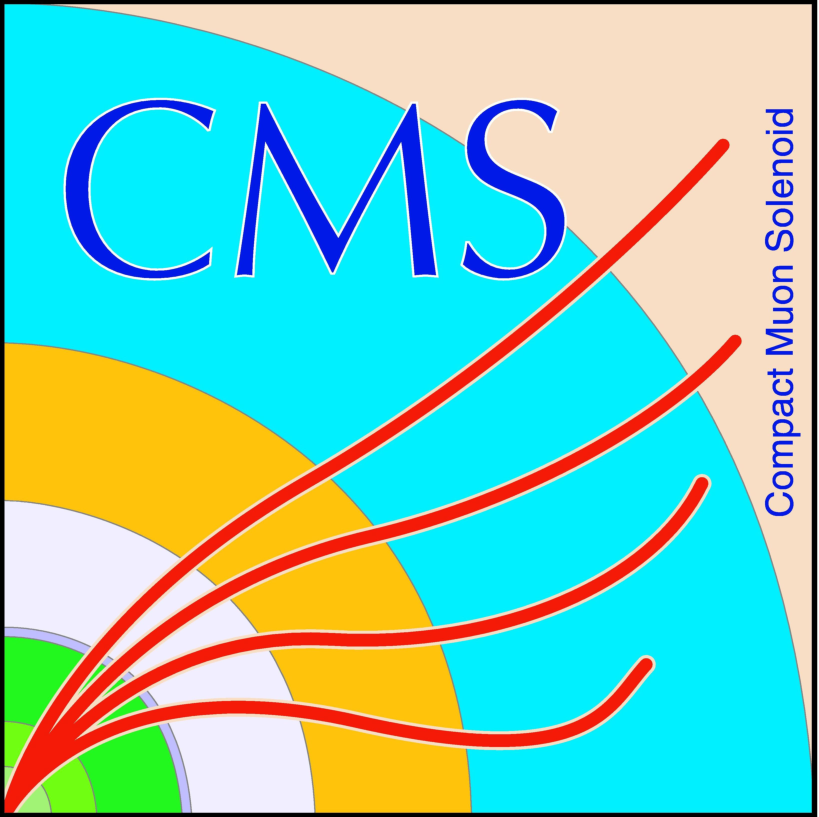
\includegraphics[width=0.05\textwidth]{figures/cms_logo.pdf} &
			&
			
\includegraphics[width=0.05\textwidth]{figures/atlas_logo.pdf} 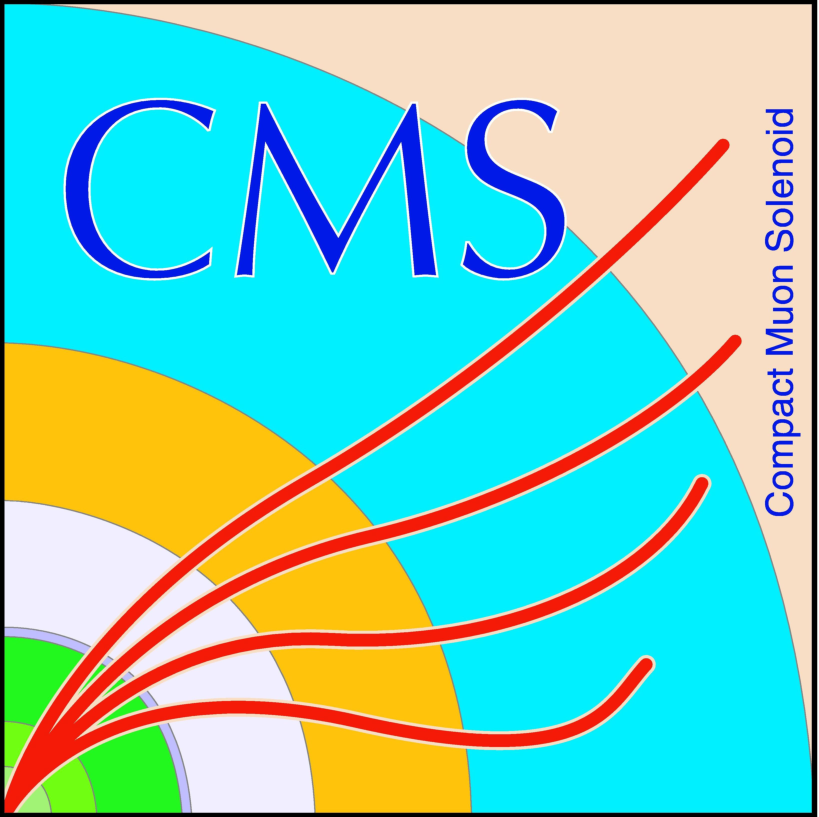
\includegraphics[width=0.05\textwidth]{figures/cms_logo.pdf} 	
			\\
			$ee$ &
			
\includegraphics[width=0.05\textwidth]{figures/atlas_logo.pdf} &
			
\includegraphics[width=0.05\textwidth]{figures/atlas_logo.pdf} &
			
\includegraphics[width=0.05\textwidth]{figures/atlas_logo.pdf} &
			
\includegraphics[width=0.05\textwidth]{figures/atlas_logo.pdf} &
			&
			
\includegraphics[width=0.05\textwidth]{figures/atlas_logo.pdf} 	
			\\	


			
			\hline
			$\tau_{had} \tau_{had}$ &
			
\includegraphics[width=0.05\textwidth]{figures/atlas_logo.pdf} 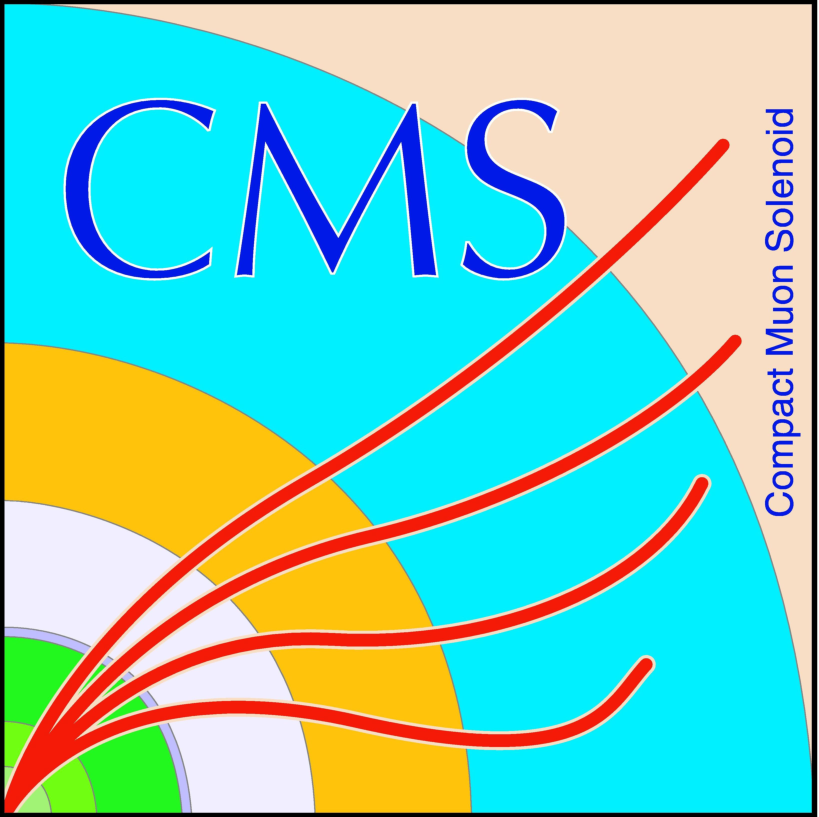
\includegraphics[width=0.05\textwidth]{figures/cms_logo.pdf} &
			
\includegraphics[width=0.05\textwidth]{figures/atlas_logo.pdf} 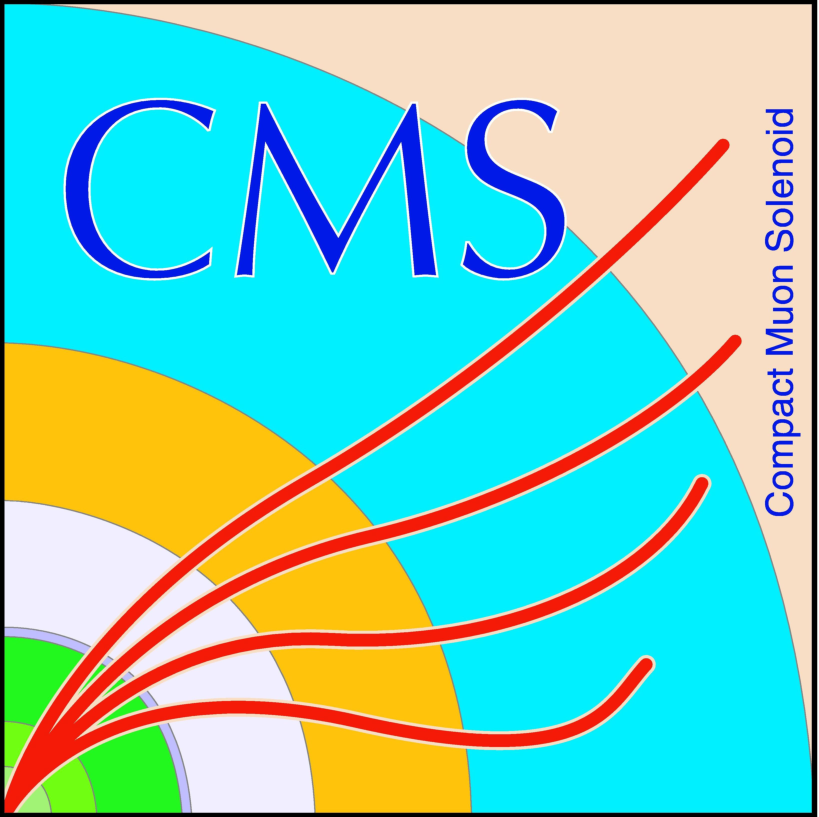
\includegraphics[width=0.05\textwidth]{figures/cms_logo.pdf} &	
			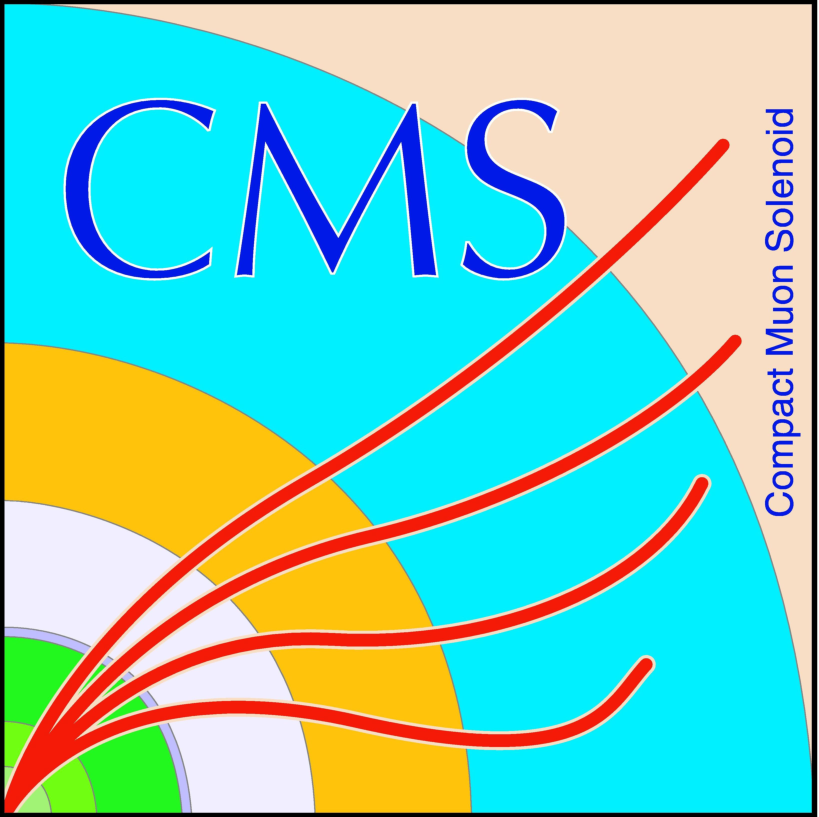
\includegraphics[width=0.05\textwidth]{figures/cms_logo.pdf}&
			&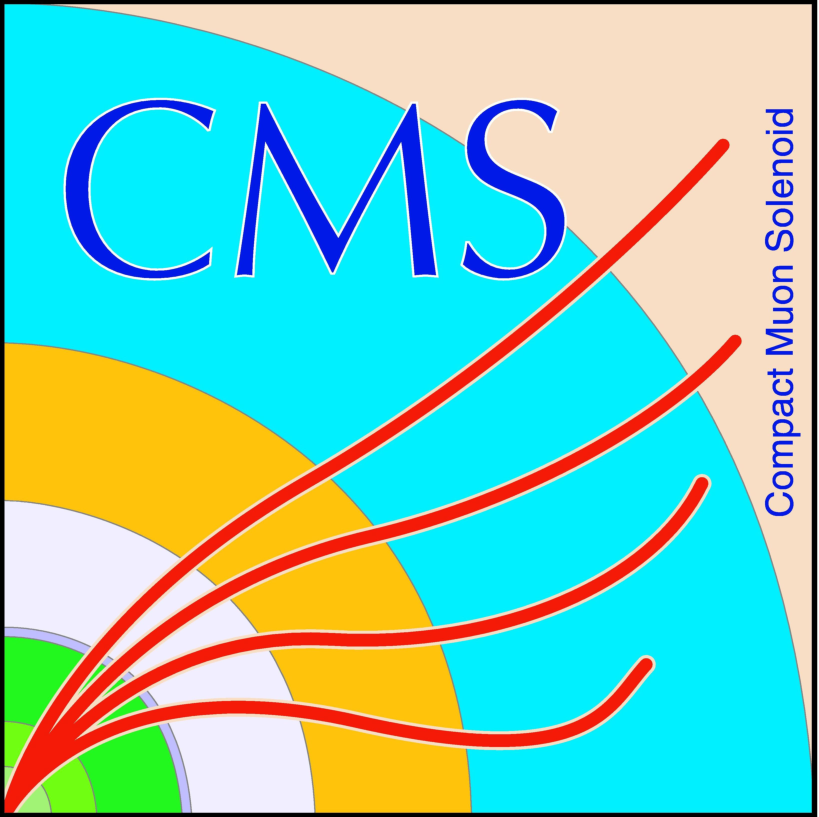
\includegraphics[width=0.05\textwidth]{figures/cms_logo.pdf} 
			&  
			\\					
				
		\end{tabular}
	\end{table}
	\scriptsize
	$^*$ ATLAS: 7 TeV only; CMS: control region only \\
	NB: Analysis definitions not identical between collaborations!  See notes for more detail
\end{frame}


\begin{frame}{$H \rightarrow \tau\tau$: $\tau_{lep}\tau_{lep}$ VBF}
	\begin{columns}[c]
		\column{0.4\textwidth}
			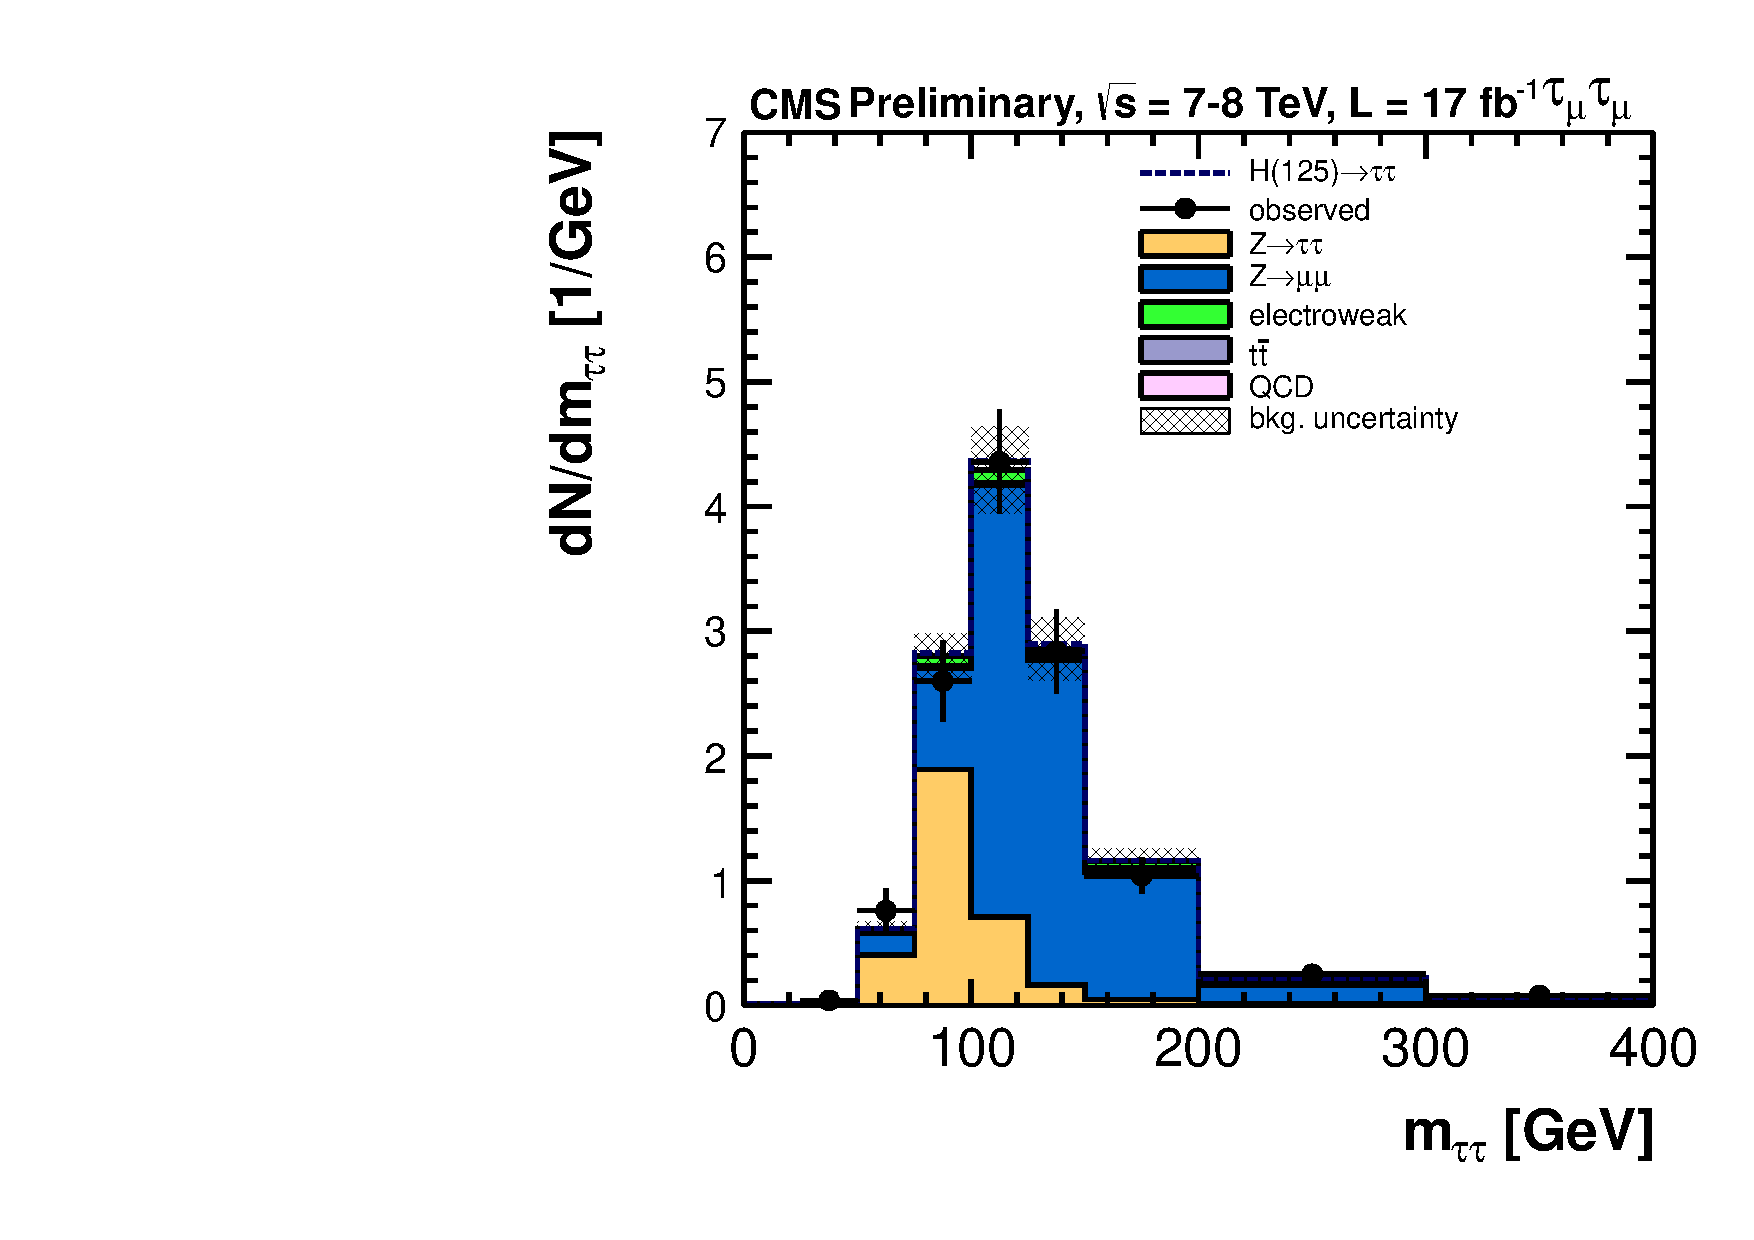
\includegraphics[width=0.92\textwidth]{figures/cms_htautau_mumu_VBF.pdf} \\	
		\column{0.2\textwidth} \scriptsize
			CMS breaks down results by final state of $\tau$`s ($\mu \mu$ vs. $e\mu$) \\ 
			\textcolor{BrickRed}{7 TeV and 8 TeV data combined}
		\column{0.4\textwidth}	
			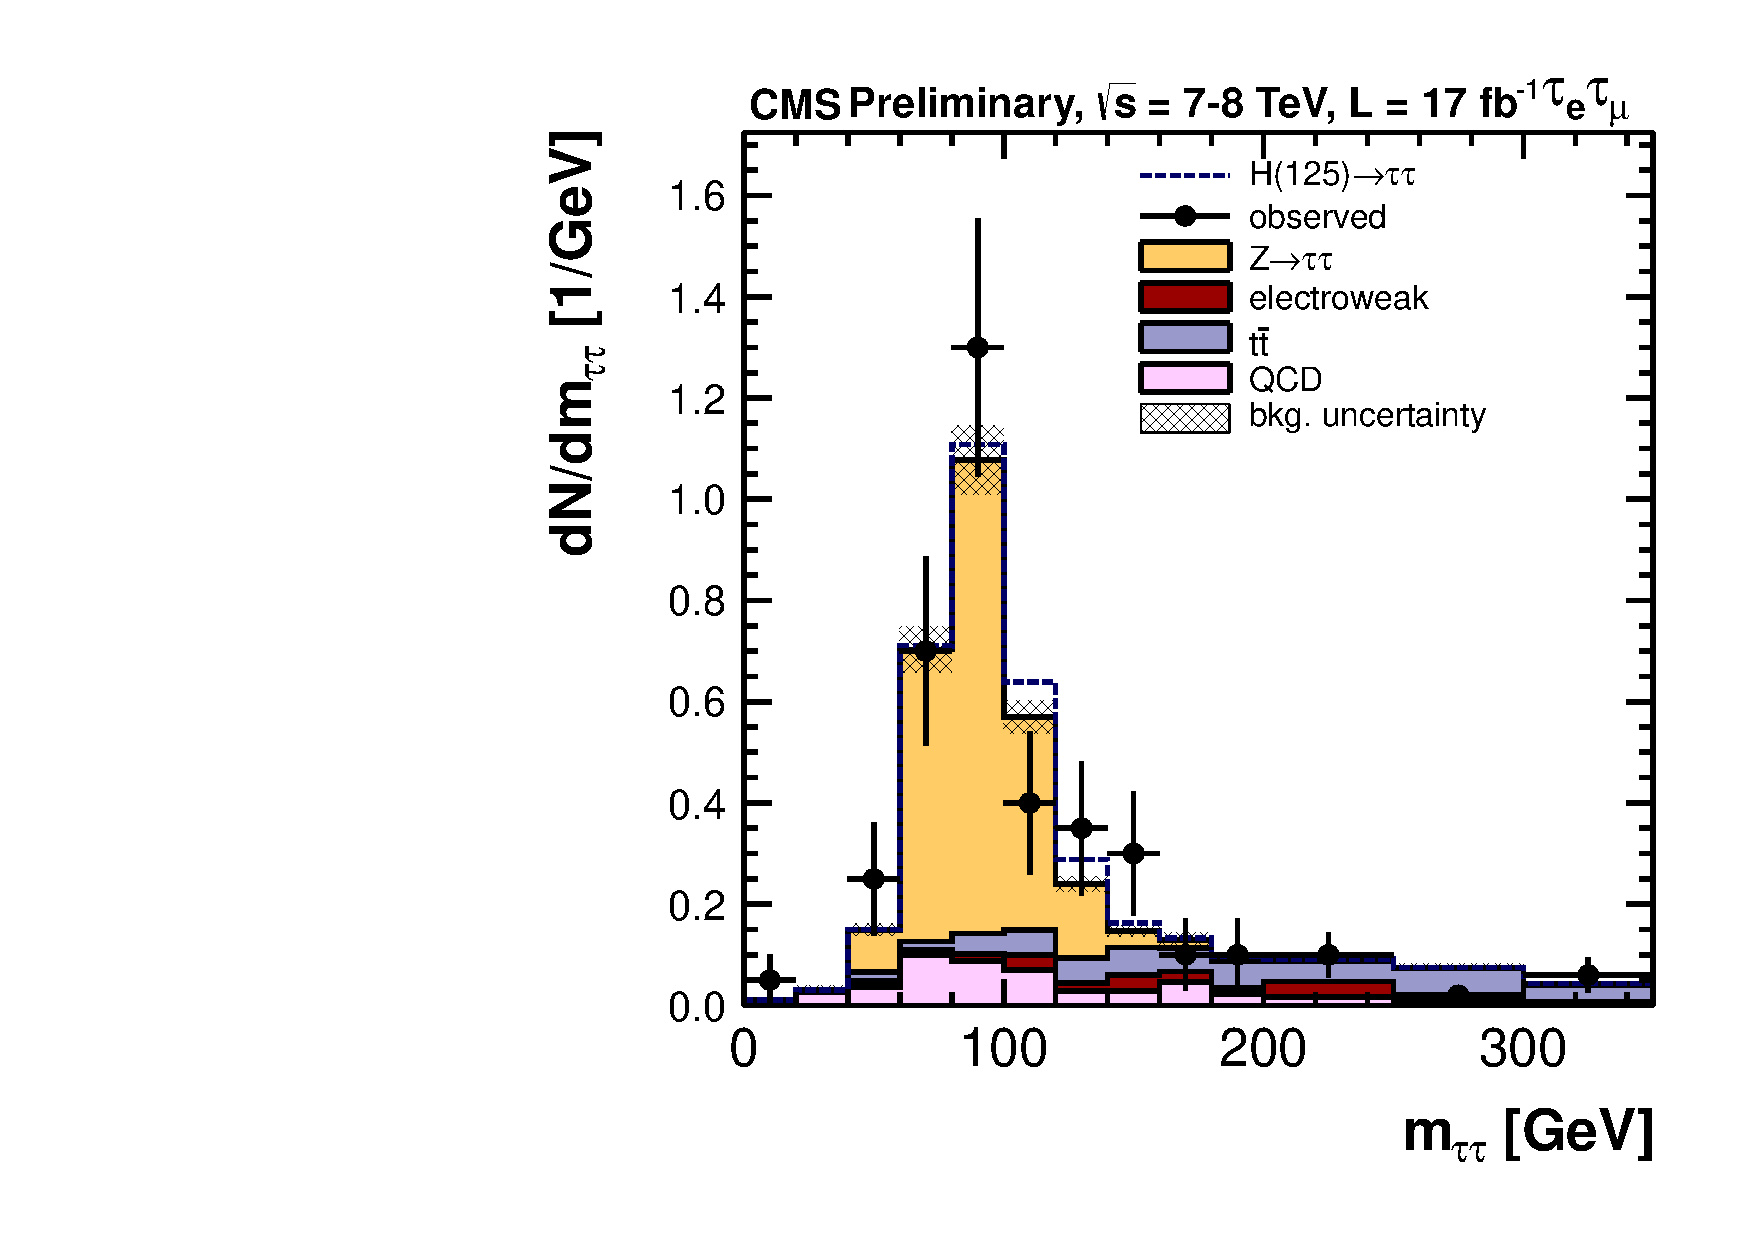
\includegraphics[width=0.92\textwidth]{figures/cms_htautau_emu_VBF.pdf}	
	\end{columns}
	
	\begin{center}
	\line(1,0){250}
	\end{center}
	
	\begin{columns}[c]
		\column{0.4\textwidth}
			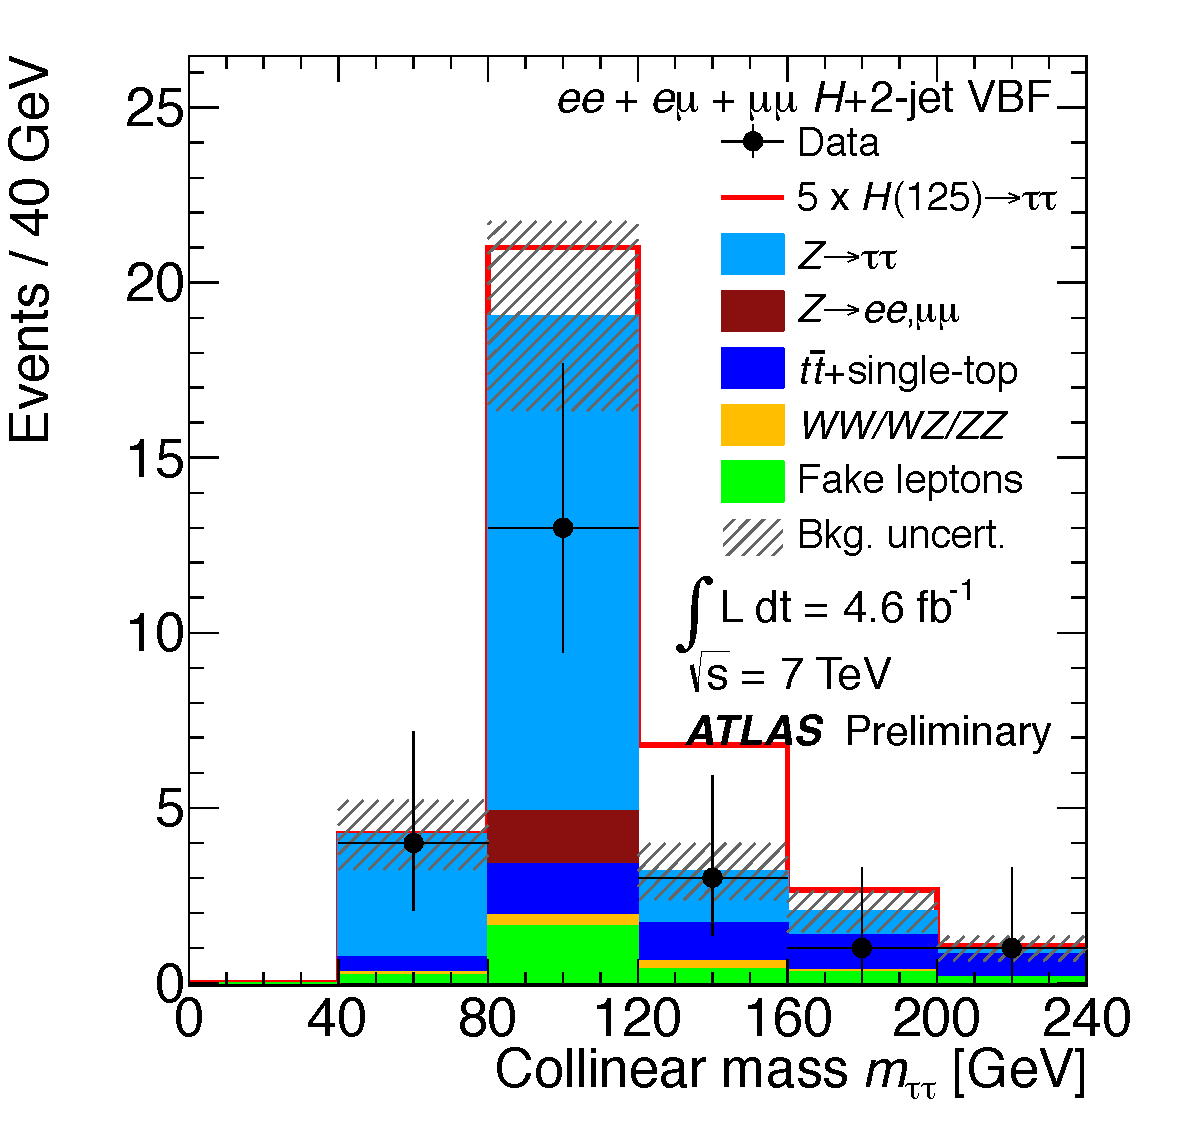
\includegraphics[width=0.92\textwidth]{figures/atlas_htautau_leplep_VBF_7TeV.pdf}		
		\column{0.2\textwidth} \scriptsize
				ATLAS breaks down results by energy (7 TeV vs. 8 TeV) \\
				\textcolor{BrickRed}{$\tau$ final states combined ($ee$, $e\mu$, $\mu\mu$)}
		\column{0.4\textwidth}
			\includegraphics[width=0.92\textwidth]{figures/atlas_htautau_leplep_VBF_8TeV.pdf} 
	\end{columns}
\end{frame}






\begin{frame}{$H\rightarrow \tau \tau$: CMS Sensitivity}
	\begin{columns}[c]
		\column{0.5\textwidth}
			\includegraphics[width=0.9\textwidth]{/Users/caitlinmalone/Documents/ATLAS/HiggsCouplings2013/figures/cms_htautau_bkg_only_brazil.pdf}\\
		\column{0.5\textwidth}
			\includegraphics[width=0.9\textwidth]{/Users/caitlinmalone/Documents/ATLAS/HiggsCouplings2013/figures/cms_htautau_sig_plus_bkg_brazil.pdf}\\
	\end{columns}	
	
	\begin{columns}
		\column{0.5\textwidth}
			\scriptsize 
			At $m_H$=125 GeV, observed (expected) 95\% CL upper limits on cross section to 1.0 (1.63) $\times$ SM (background-only hypothesis)
		\column{0.5\textwidth}
			\scriptsize
			Includes an SM Higgs boson at $m_H$=125 GeV for the expected result 
	\end{columns}	

\end{frame}


\begin{frame}{$H\rightarrow \tau \tau$: CMS Channel Breakdown}
	\includegraphics[width=\textwidth]{/Users/caitlinmalone/Documents/ATLAS/HiggsCouplings2013/figures/cms_htautau_signal_strength.pdf}
\end{frame}



\begin{frame}{$H\rightarrow\tau\tau$: ATLAS Sensitivity}
	\begin{columns}[c]
		\column{0.5\textwidth}
			\includegraphics[width=\textwidth]{/Users/caitlinmalone/Documents/ATLAS/HiggsCouplings2013/figures/atlas_htautau_brazil.pdf}
		\column{0.5\textwidth}
			\includegraphics[width=\textwidth]{/Users/caitlinmalone/Documents/ATLAS/HiggsCouplings2013/figures/atlas_htautau_p_value.pdf}
	\end{columns}
	\scriptsize
	for $m_H$=125 GeV, local significance of 1.1$\sigma$ and best fit value $\mu$=0.7$\pm$0.7
\end{frame}


\begin{frame}{$H\rightarrow\tau\tau$: ATLAS Channel Breakdown}
	\begin{columns}[c]
		\column{0.33\textwidth}
			\includegraphics[width=0.9\textwidth]{/Users/caitlinmalone/Documents/ATLAS/HiggsCouplings2013/figures/atlas_htautau_leplep_brazil.pdf}\\
			\scriptsize\center \vspace{-0.5cm}
			$\tau_{lep}\tau_{lep}$
		\column{0.33\textwidth}
			\includegraphics[width=0.9\textwidth]{/Users/caitlinmalone/Documents/ATLAS/HiggsCouplings2013/figures/atlas_htautau_lephad_brazil.pdf} 
			\scriptsize\center \vspace{-0.5cm}
			$\tau_{lep}\tau_{had}$
		\column{0.33\textwidth}
			\includegraphics[width=0.9\textwidth]{/Users/caitlinmalone/Documents/ATLAS/HiggsCouplings2013/figures/atlas_htautau_hadhad_brazil.pdf} 
			\scriptsize \center \vspace{-0.5cm}
			$\tau_{had}\tau_{had}$
	\end{columns}
	
	\begin{center}
	\line(1,0){250}
	\end{center}
	
	\begin{columns}[c]
		\column{0.5\textwidth}
%			\includegraphics[width=0.7\textwidth]{/Users/caitlinmalone/Documents/ATLAS/HiggsCouplings2013/figures/atlas_htautau__brazil.pdf}\\
			\scriptsize \center \vspace{-0.5cm}
			VBF channels
		\column{0.5\textwidth}
%			\includegraphics[width=0.7\textwidth]{/Users/caitlinmalone/Documents/ATLAS/HiggsCouplings2013/figures/atlas_htautau_lephad_brazil.pdf} \\
			\scriptsize \center \vspace{-0.5cm}
			non-VBF channels
	\end{columns}

\end{frame}



\begin{frame}{$H\rightarrow bb$ Motivation}
	\begin{itemize}
		\item High branching ratio (about 58\%) means that observation is crucial 
		\item Direct ggF impossible to observe because of high QCD background
		\begin{itemize}
			\item VH: associated production
			\item ttH: allows us to measure couplings to quarks?
			\item VBF: tag the forward jets
		\end{itemize}
	\end{itemize}
\end{frame}


\begin{frame}{Higgs to bb at ATLAS}
	\begin{itemize}
		\item VH: sensitivity of 1.8 times SM
		\item ttH: sensitivity of 13.1 times SM
		\item VBF: result planned for winter 2015
	\end{itemize}
\end{frame}


\begin{frame}{Higgs to bb at CMS}
	\begin{itemize}
		\item VH: 2.1 sigma excess observed
		\item ttH: done in combination with $\tau \tau$
		\item VBF: sensitivity 3.6 times SM
	\end{itemize}
\end{frame}



% http://cds.cern.ch/record/1523695/files/ATLAS-CONF-2013-010.pdf
\begin{frame}{$H\rightarrow\mu \mu$ Motivation}
	\begin{itemize}
		\item Small cross section
		\item Clean final state signature
		\item Only channel for measuring coupling to second-generation fermions
		\item Large irreducible background of $Z/\gamma^*\rightarrow\mu\mu$
		\item Can have enhanced BF from non-SM contributions
	\end{itemize}
\end{frame}




\begin{frame}{Higgs to $\mu \mu$ at ATLAS}
	\begin{columns}[c]
	\column{2.5in}
		\begin{itemize}  \scriptsize
			\item \textcolor{BrickRed}{Reconstruct invariant mass of 2 muons, $p_{T}^{\mu_1}>25$ GeV and $p_{T}^{\mu_2}>15$ GeV}
			\item Remove 60\% of Drell-Yan background events (and keeping 80\% of signal) by requiring p$_T^{\mu+\mu-}>$ 15 GeV (events failing this cut go into a background control region)
			\item Search for bump in the invariant mass spectrum, main background is Z+jets
			\item Background model: exponential plus Breit-Wigner, to capture Z tail
		\end{itemize}
	\column{2.5in}
			\includegraphics[width=0.7\textwidth]{/Users/caitlinmalone/Documents/ATLAS/HiggsCouplings2013/figures/atlas_hmumu_mass_linear.pdf} \\
%			\includegraphics[width=0.7\textwidth]{/Users/caitlinmalone/Documents/ATLAS/HiggsCouplings2013/figures/atlas_hmumu_mass_log.pdf}			
	\end{columns}
	\begin{columns}[c]
		\column{0.25\textwidth}
			\includegraphics[width=1.1\textwidth]{/Users/caitlinmalone/Documents/ATLAS/HiggsCouplings2013/figures/atlas_hmumu_mass_sim_central.pdf}
		\column{0.25\textwidth}
			\includegraphics[width=1.1\textwidth]{/Users/caitlinmalone/Documents/ATLAS/HiggsCouplings2013/figures/atlas_hmumu_mass_data_central.pdf}
		\column{0.25\textwidth}
			\includegraphics[width=1.1\textwidth]{/Users/caitlinmalone/Documents/ATLAS/HiggsCouplings2013/figures/atlas_hmumu_mass_sim_non_central.pdf}
		\column{0.25\textwidth}
			\includegraphics[width=1.1\textwidth]{/Users/caitlinmalone/Documents/ATLAS/HiggsCouplings2013/figures/atlas_hmumu_mass_data_non_central.pdf}
	\end{columns}
	\begin{columns}[c]
		\column{0.5\textwidth}
		\tiny{Simulation and data in central region ($|\eta(\mu_{1,2})|<1.0$), fit with BW + exponential}
		\column{0.5\textwidth}
		\tiny{Simulation and data in non-central region ($|\eta(\mu_{1,2})|>1.0$), fit with BW + exponential}
	\end{columns}
	
\end{frame}


\begin{frame}{$H\rightarrow\mu\mu$ Results at ATLAS}
	\begin{columns}
		\column{2.5in}
			\includegraphics[width=0.9\textwidth]{/Users/caitlinmalone/Documents/ATLAS/HiggsCouplings2013/figures/atlas_hmumu_brazil.pdf}
		\column{2.5in}
			\includegraphics[width=0.9\textwidth]{/Users/caitlinmalone/Documents/ATLAS/HiggsCouplings2013/figures/atlas_hmumu_p_value.pdf}			
	\end{columns}
	
	\begin{table}
	\scriptsize
	\begin{tabular}{c | c | c | c | c | c | c } 
	\hline 
	$m_H$ & observed limits & exp. median & exp. + 2$\sigma$ & exp. +1$\sigma$ & exp. -1$\sigma$ & exp. -2$\sigma$ \\ \hline
	110 & 5.1 & 10.4 & 20.0 & 14.6 & 7.5 & 5.6 \\
	115 & 5.7 & 7.5 & 14.5 & 10.6 & 5.4 & 4.0 \\
	120 & 9.2 & 7.6 & 14.6 & 10.7 & 5.5 & 4.1 \\
	125 & 9.8 & 8.2 & 15.9 & 11.6 & 5.9 & 4.4 \\
	130 & 10.8 & 9.1 & 17.5 & 12.8 & 6.5 & 4.9 \\
	135 & 11.0 & 10.4 & 20.1 & 14.6 & 7.5 & 5.6 \\
	140 & 16.8 & 12.9 & 25.0 & 18.2 & 9.3 & 6.9 \\
	145 & 16.9 & 18.3 & 35.3 & 25.7 & 13.2 & 9.8 \\
	150 & 22.1 & 31.3 & 60.6 & 44.2 & 22.6 & 16.8 \\ \hline
	\end{tabular}
	\end{table}
\end{frame}


\begin{frame}{$H\rightarrow\mu\mu$ Results at CMS}
to be included if approved
\end{frame}



\begin{frame}{Prospects for 2015 and beyond}

\end{frame}



\begin{frame}{References}
	\begin{itemize} \scriptsize
		\item ATLAS, \href{https://atlas.web.cern.ch/Atlas/GROUPS/PHYSICS/CONFNOTES/ATLAS-CONF-2013-079/}{ \textit{Search for the bb decay of the Standard Model Higgs boson in associated (W/Z)H production with the ATLAS detector}}, 19 July 2013
		\item ATLAS, \href{https://atlas.web.cern.ch/Atlas/GROUPS/PHYSICS/CONFNOTES/ATLAS-CONF-2012-135/}{\textit{Search for the Standard Model Higgs boson produced in association with top quarks in proton-proton collisions at $\sqrt s$=7 TeV using the ATLAS detector}}, 15 September 2012
		\item CMS, \href{http://cds.cern.ch/record/1546801?ln=en}{\textit{Search for the SM Higgs boson produced in association with W or Z bosons, and decaying to bottom quarks}}, 14 May 2013
		\item CMS, \href{http://cds.cern.ch/record/1564682?ln=en}{\textit{Search for Higgs Boson Production in association with a top-quark pair and decaying to bottom quarks or tau leptons}}, 26 July 2013
		\item ATLAS, \href{https://atlas.web.cern.ch/Atlas/GROUPS/PHYSICS/CONFNOTES/ATLAS-CONF-2012-160/}{\textit{Search for the Standard Model Higgs boson in H to tau tau decays in proton-proton collisions with the ATLAS detector}}, 13 November 2012
		\item CMS, \href{https://cds.cern.ch/record/1528271?ln=en}{\textit{Search for the standard model Higgs boson decaying to tau pairs in proton-proton collisions at $\sqrt s$=7 and 8 TeV}}, 15 March 2013
		\item CMS, \href{https://cds.cern.ch/record/1528147/files/HIG-12-053-pas.pdf}{\textit{Search for the standard model Higgs boson decaying to tau pairs produced in association with a W or Z boson with the CMS experiment in pp collisions at $\sqrt s$ = 7 and 8 TeV}}
		\item ATLAS, \href{https://atlas.web.cern.ch/Atlas/GROUPS/PHYSICS/CONFNOTES/ATLAS-CONF-2013-010/}{\textit{Search for the SM Higgs boson in H to mu mu decays with the ATLAS detector}}, 5 March 2013
		\item LHC Higgs Cross Section Working Group, \href{Handbook of LHC Higgs Cross Sections: 1. Inclusive Observables}{\textit{http://arxiv.org/abs/1101.0593}}, 20 May 2011
		\item LHC Higgs Cross Section Working Group, \href{http://arxiv.org/abs/1201.3084}{\textit{Handbook of LHC Higgs Cross Sections: 2. Differential Distributions}}
	\end{itemize}
\end{frame}


\end{document}
